% TODO - revisar y redactar todo el capítulo
\section{Resultados obtenidos}
\label{sec:resultados}

Este capítulo presenta los resultados de la validación del sistema en dos entornos complementarios: el banco de ensayo Arduino, que permitió reproducir condiciones adversas de forma controlada, y un vehículo real, en el que se verificó la interoperabilidad del sistema con una ECU de producción a través del conector OBD-II estándar. Los resultados se organizan en torno a cuatro dimensiones: funcionalidad del protocolo, rendimiento de la comunicación, comportamiento ante condiciones adversas y grado de consecución de los objetivos planteados en el Capítulo~2.

Para verificar que los resultados obtenidos por la herramienta desarrollada son verídicos, previamente se realizó un escaneo de los DTCs y una lectura de PIDs con una herramienta comercial genérica KONWEII~\cite{KONWEII_scanner} junto con la aplicación móvil Car Scanner ELM OBD2~\cite{CarScanner_app}, tomada como referencia. La Figura~\ref{fig:ref_comercial} muestra el cuadro de instrumentos y la lista de DTCs obtenidos con la herramienta de referencia, que sirvieron de patrón de comparación para validar los valores leídos por la herramienta desarrollada.

\begin{figure}[H]
\centering
\begin{minipage}[t]{0.42\textwidth}
\centering
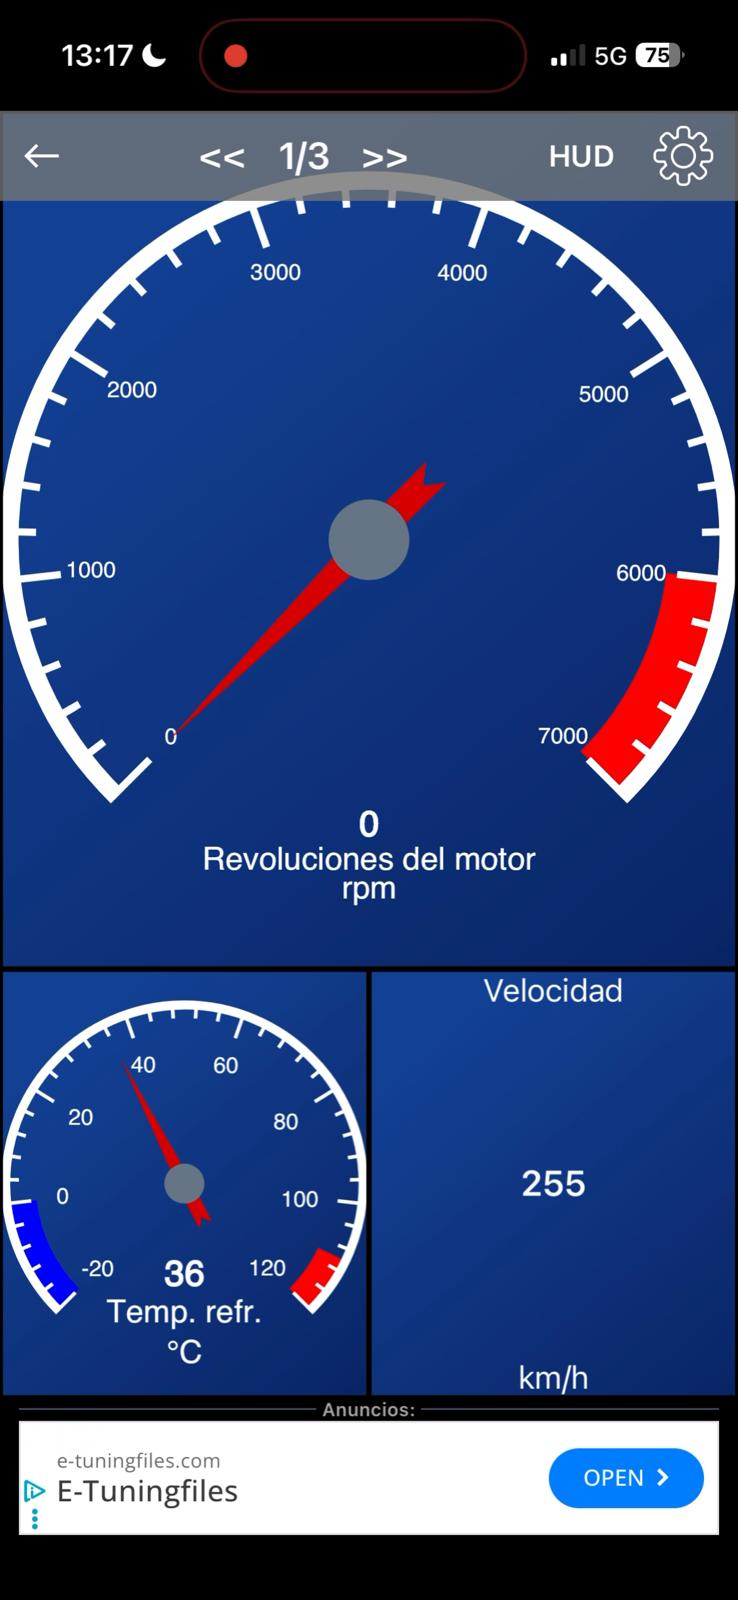
\includegraphics[height=10.5cm]{Ilustraciones/cuadro_konwei.png}
\subcaption{Cuadro de instrumentos (lectura de PIDs).}
\label{fig:ref_panel}
\end{minipage}\hfill
\begin{minipage}[t]{0.42\textwidth}
\centering
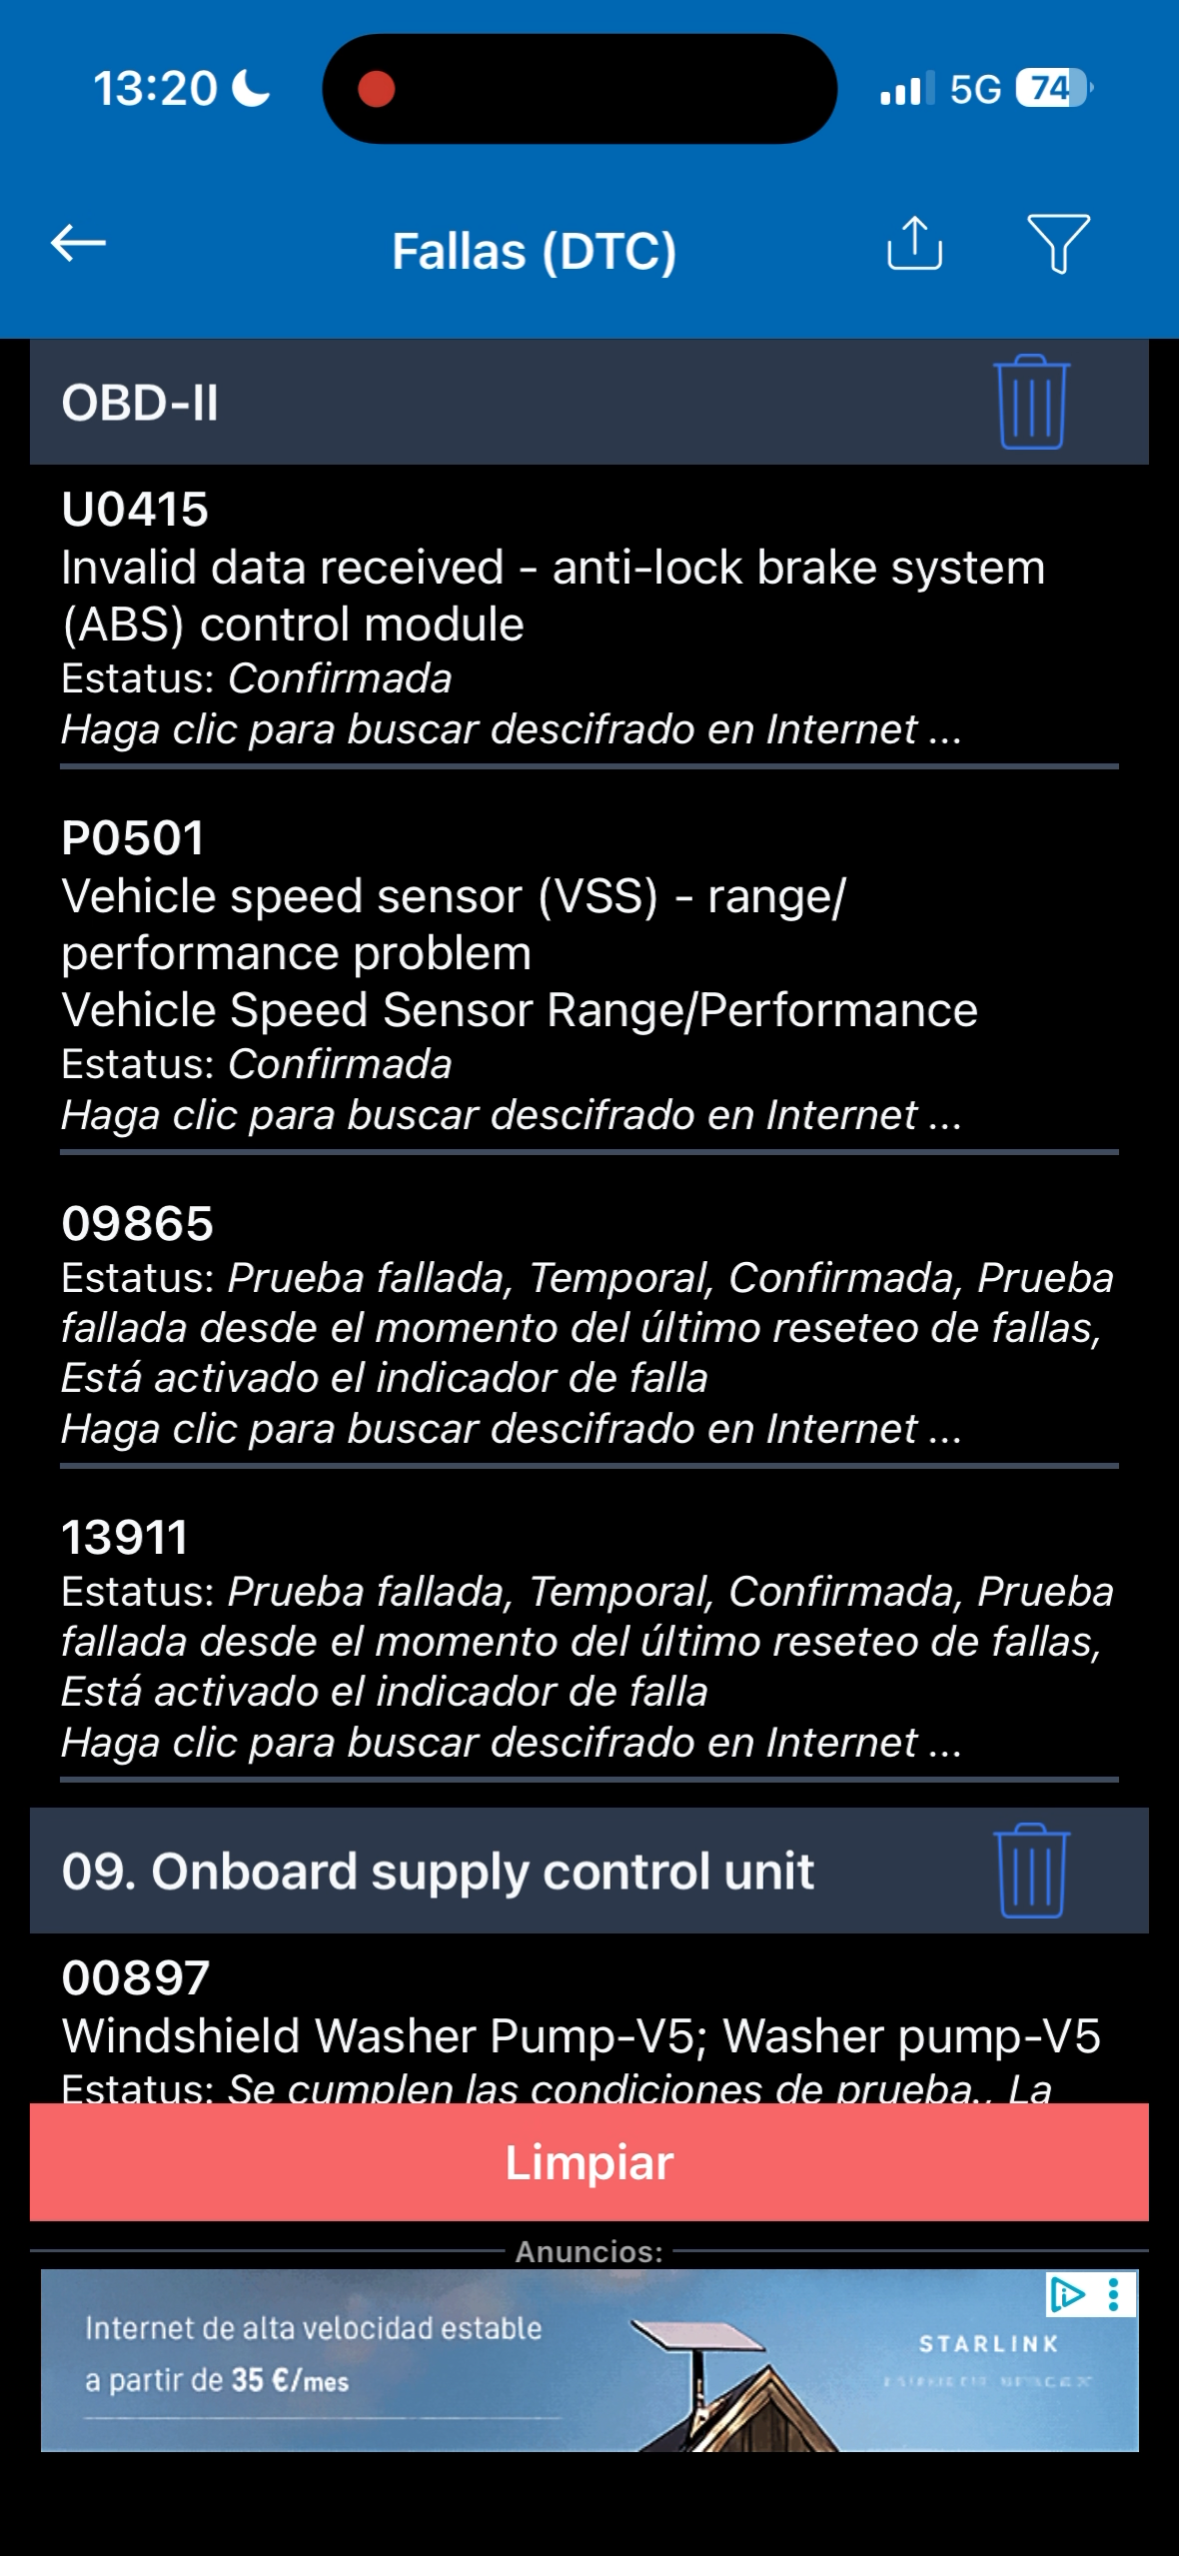
\includegraphics[height=10.5cm]{Ilustraciones/dtc_konwei.PNG}
\subcaption{Lista de DTCs.}
\label{fig:ref_dtcs}
\end{minipage}
\caption{Herramienta comercial de referencia (Car Scanner ELM OBD2~\cite{CarScanner_app}) usada como patrón de comparación: cuadro de instrumentos (a) y lista de DTCs (b).}
\label{fig:ref_comercial}
\end{figure}


\section{Validación sobre vehículo real}
\label{sec:resultados_vehiculo_real}

Tras completar la validación sobre el banco de ensayo, el sistema se probó sobre un vehículo real. El vehículo objetivo inicial era un SEAT Ibiza 6J, pero debido a que la plataforma de ese modelo no implementa el protocolo OBD-II sobre el bus CAN en los pines 6 y 14 del puerto OBD, la validación final se realizó sobre un \textbf{Škoda Yeti de 2015}, perteneciente igualmente al grupo VAG y, por tanto, representativo de la misma arquitectura de diagnóstico. La conexión se efectuó mediante un cable OBD-II estándar que nos revela todos los pines del puerto de diagnóstico del vehículo: la Raspberry Pi actuó como interfaz entre el bus CAN del vehículo conectado a través de los pines 6 y 14 (\texttt{CAN\_L} y \texttt{CAN\_H} respectivamente) del puerto OBD-II y la aplicación móvil, manteniendo exactamente el mismo stack de software validado en el banco (\texttt{IsoTpTransport} sobre SocketCAN, servidor BLE GATT con NUS y aplicación React Native).

La conexión al vehículo demostró que el protocolo OBD-II implementado es compatible con ECUs de producción: la herramienta fue capaz de consultar los PIDs del modo 0x01 soportados por el vehículo, leer el VIN real mediante la secuencia ISO-TP multi-frame y recibir datos de telemetría en tiempo real a través de la aplicación móvil. Las respuestas del vehículo presentaron tiempos de respuesta ligeramente superiores a los del simulador (10--30\,ms frente a 2--8\,ms).

\begin{figure}[!htbp]
\centering
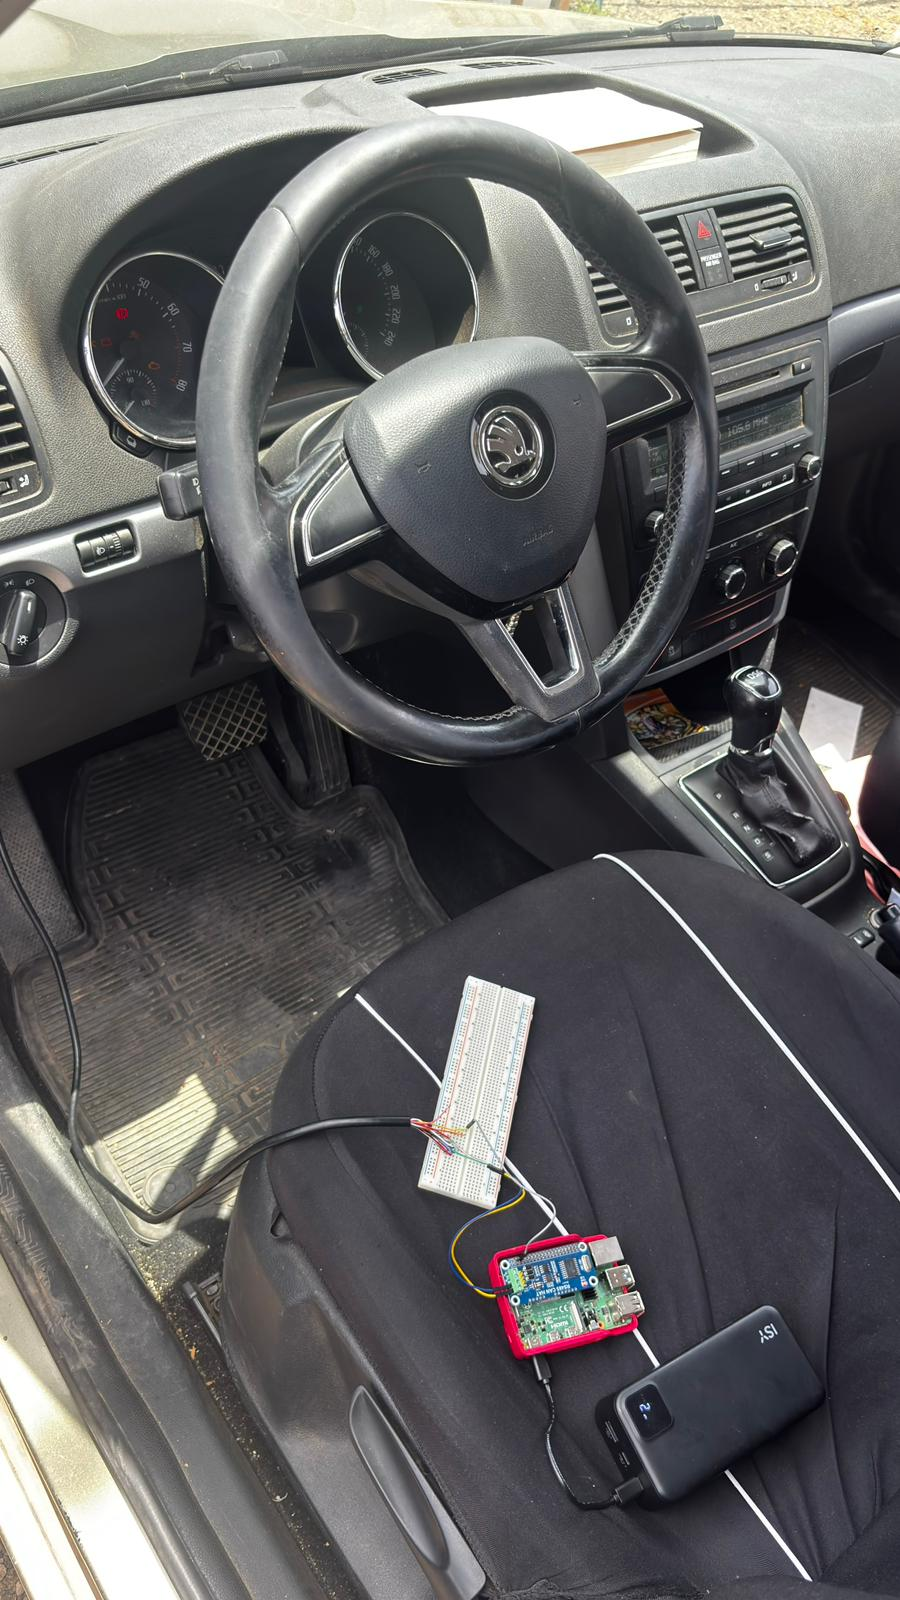
\includegraphics[width=0.45\textwidth]{Ilustraciones/foto_coche_pi.jpeg}
\caption{Sistema montado en el vehículo real: cable OBD-II conectado al puerto de diagnóstico, Raspberry Pi.}
\label{fig:vehiculo_real}
\end{figure}

Los datos leídos del Škoda Yeti se almacenaron en la base de datos SQLite como una sesión más, lo que permitió revisar a posteriori la telemetría capturada desde la propia aplicación móvil. La Figura~\ref{fig:skoda_sesion} muestra el detalle de la sesión registrada sobre el vehículo real: la lista de muestras agrupadas por sensor, el detalle de una muestra concreta con su valor decodificado y la lista de DTCs leídos de la ECU del vehículo.

\begin{figure}[H]
\centering
\begin{minipage}[t]{0.32\textwidth}
\centering
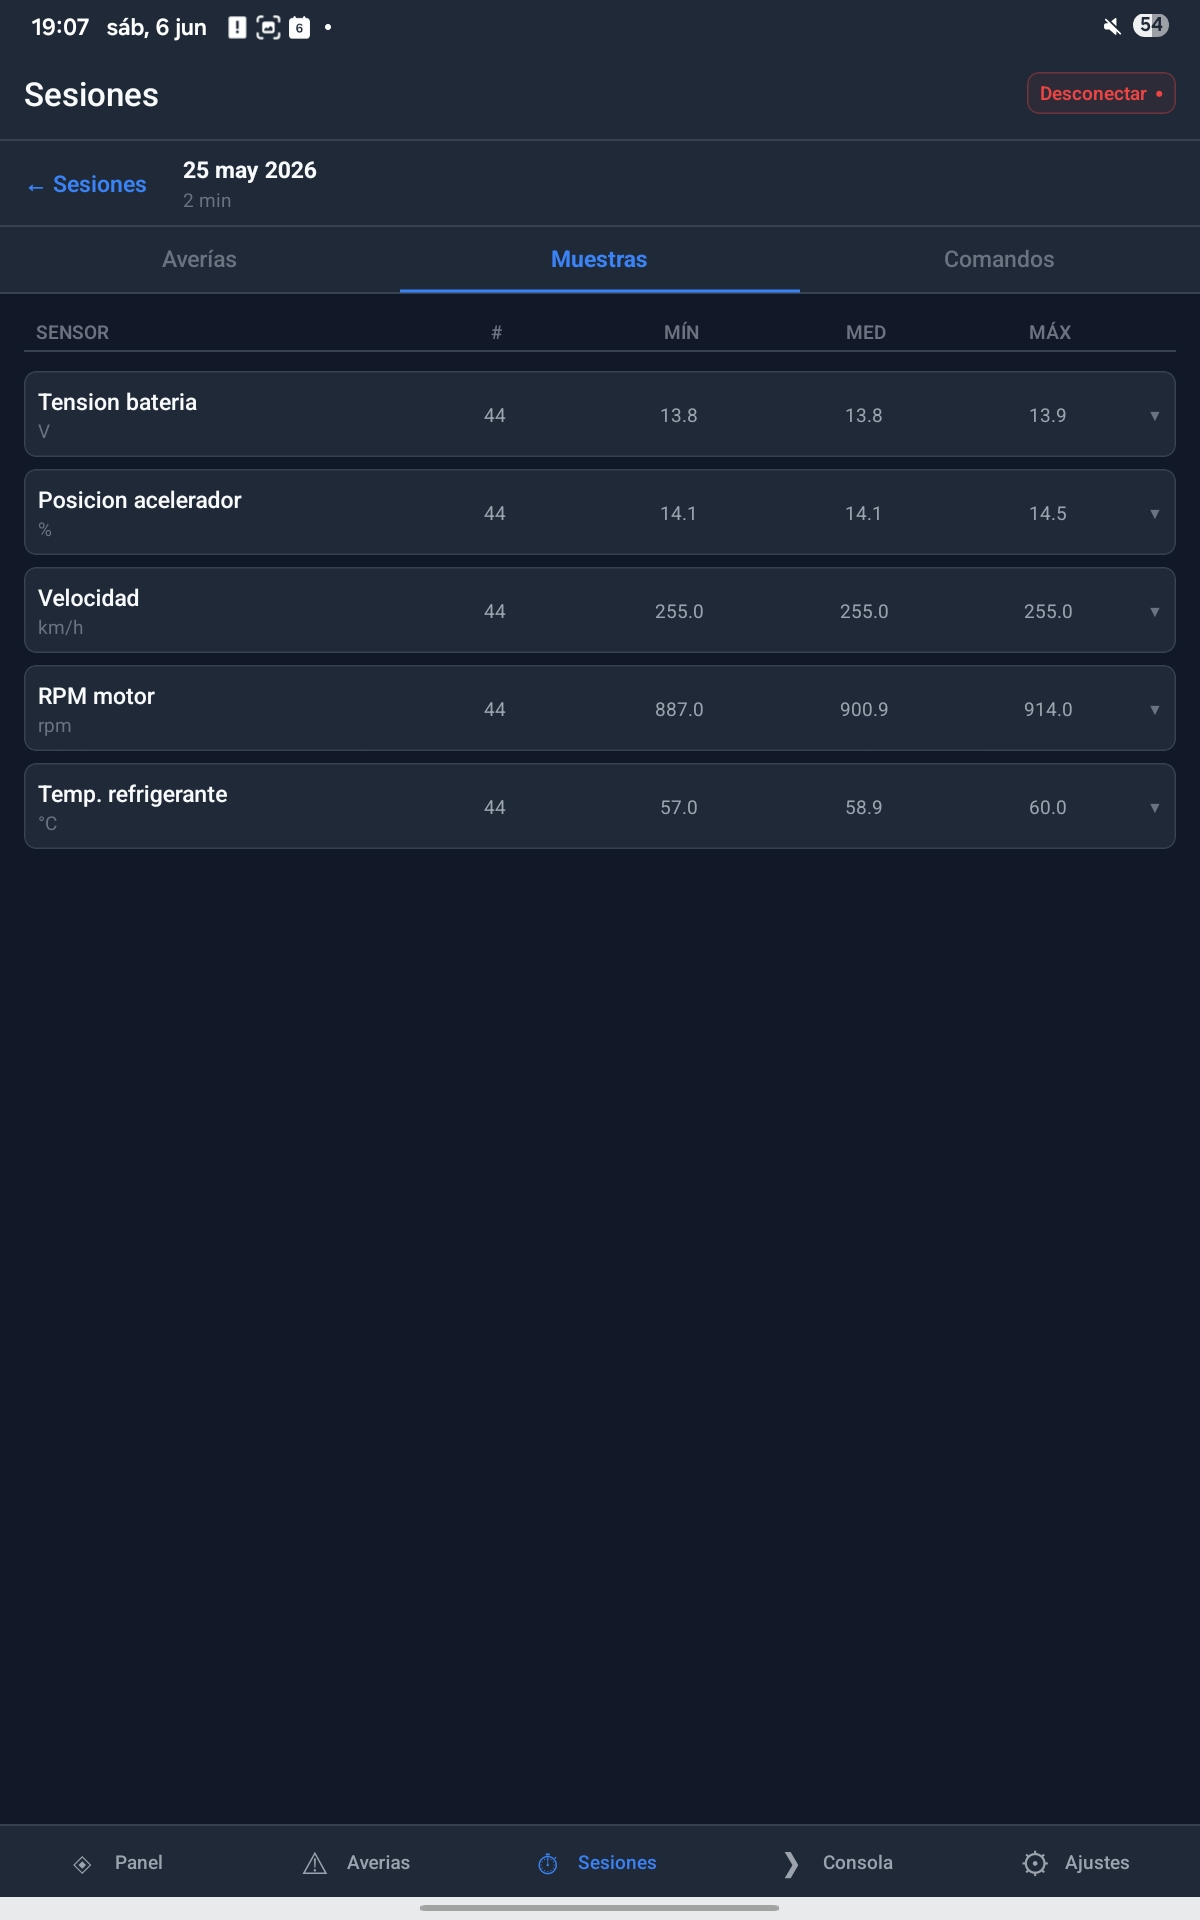
\includegraphics[height=7cm]{Ilustraciones/app_session_muestras.jpg}
\subcaption{Muestras de la sesión por sensor.}
\label{fig:skoda_muestras}
\end{minipage}\hfill
\begin{minipage}[t]{0.32\textwidth}
\centering
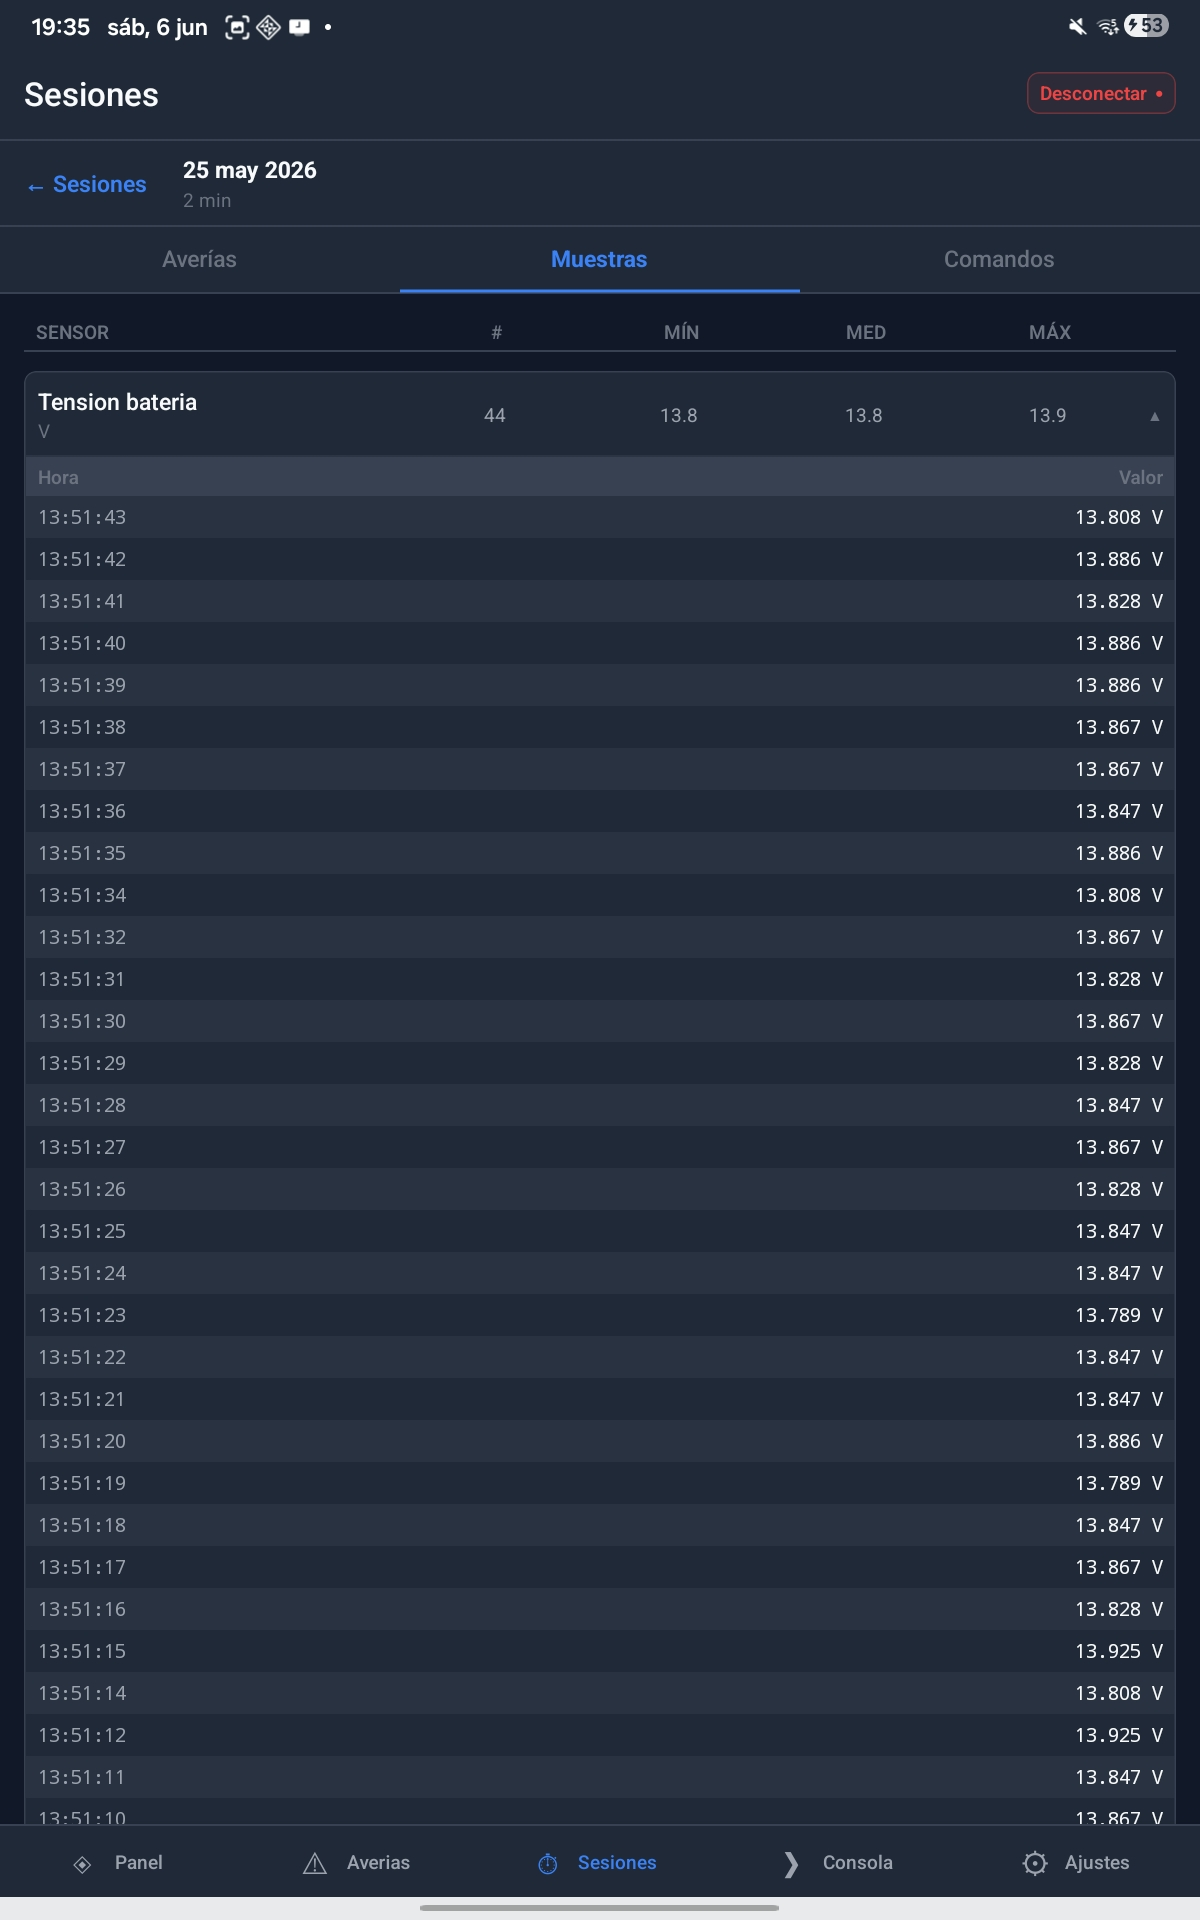
\includegraphics[height=7cm]{Ilustraciones/app_session_muestra_detalle.jpg}
\subcaption{Detalle de una muestra.}
\label{fig:skoda_muestra_detalle}
\end{minipage}\hfill
\begin{minipage}[t]{0.32\textwidth}
\centering
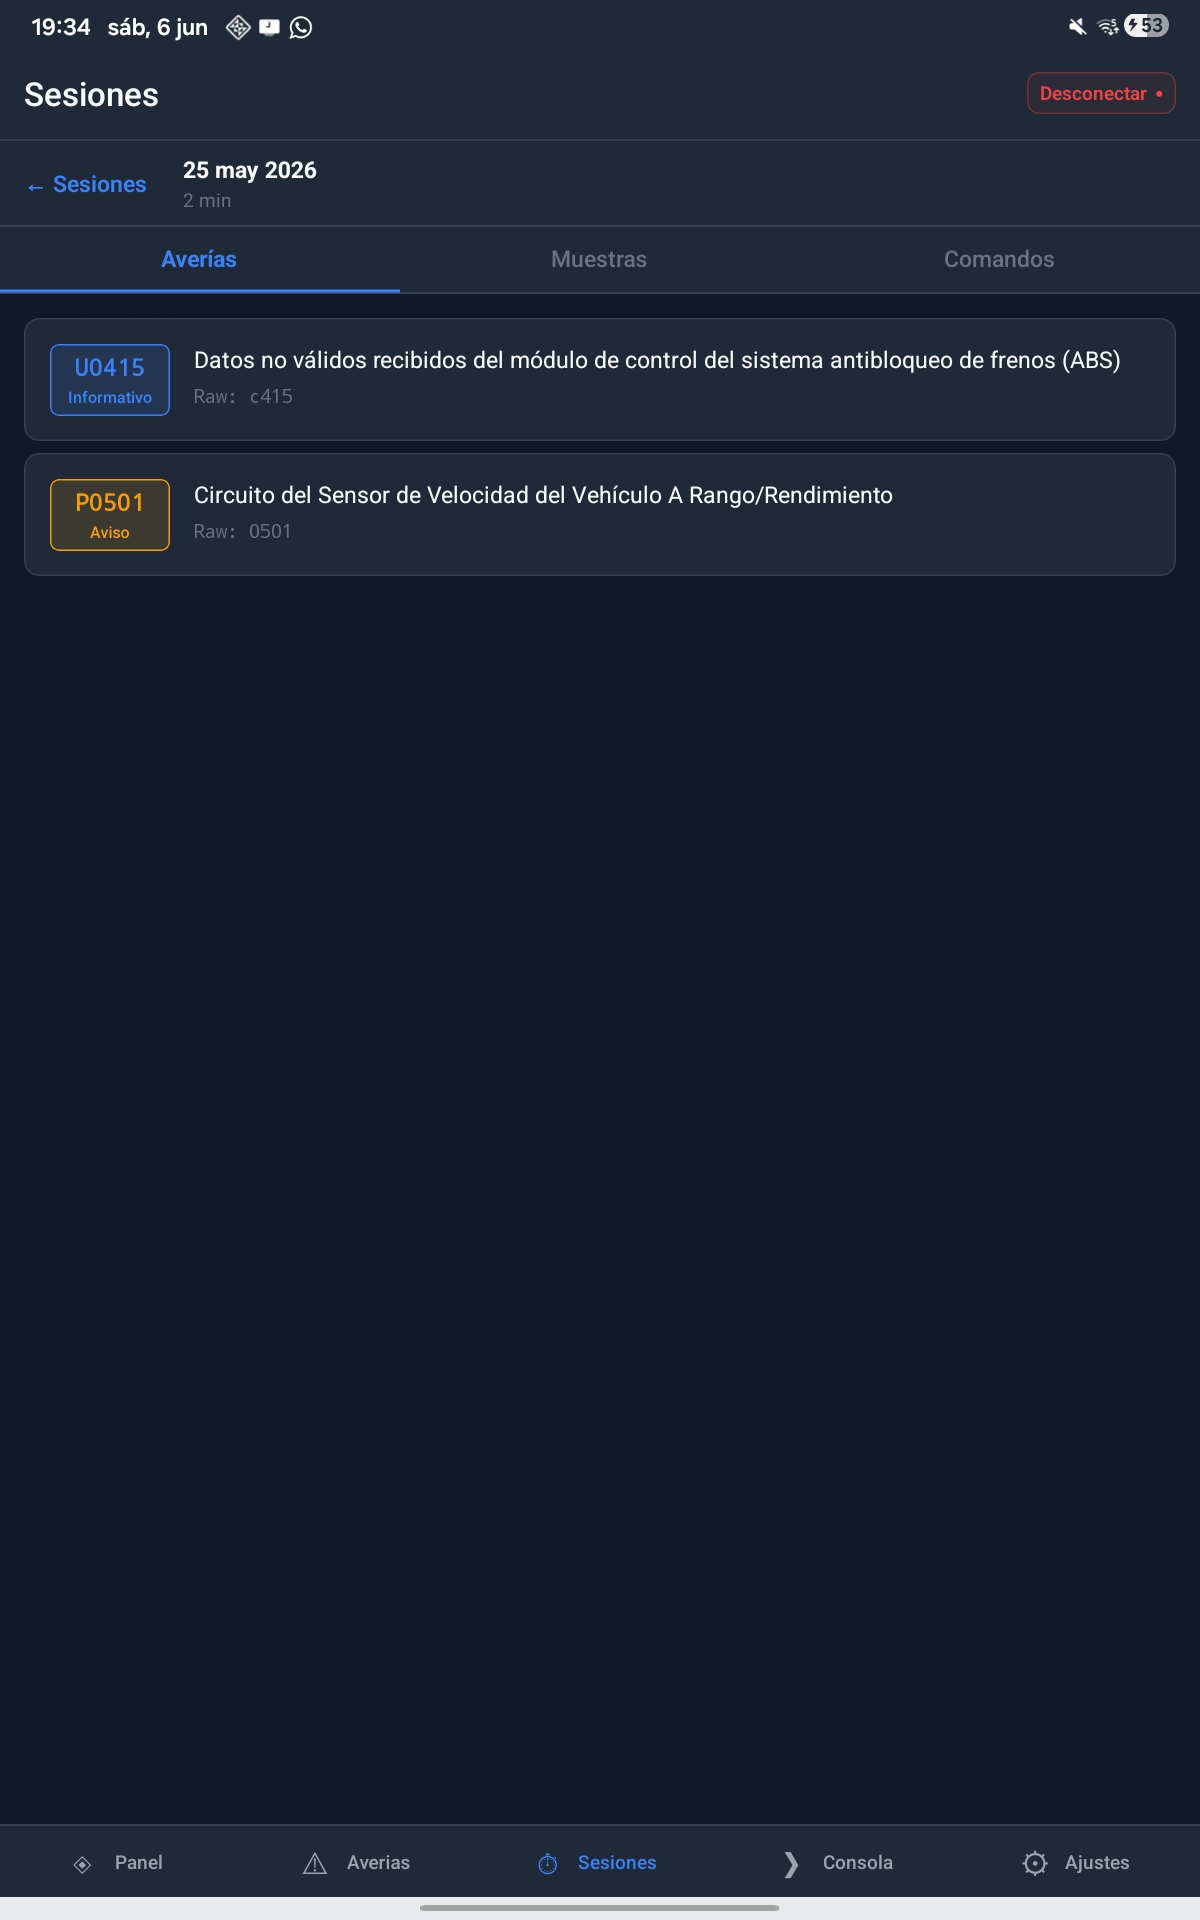
\includegraphics[height=7cm]{Ilustraciones/app_session_dtc.jpg}
\subcaption{DTCs leídos de la ECU.}
\label{fig:skoda_dtc}
\end{minipage}
\caption{Validación sobre el Škoda Yeti: detalle de la sesión registrada en SQLite, con las muestras de telemetría agrupadas por sensor (a), el detalle de una muestra concreta (b) y la lista de DTCs leídos del vehículo (c).}
\label{fig:skoda_sesion}
\end{figure}

Finalmente se realizó una prueba adicional sobre un \textbf{Opel Astra K}, perteneciente al grupo PSA/Opel y, por tanto, a una arquitectura de diagnóstico distinta a la del grupo VAG. Esta prueba corroboró el correcto funcionamiento del protocolo OBD-II: la herramienta consultó sin incidencias los PIDs del modo 0x01 y leyó el VIN del vehículo, confirmando que la capa de diagnóstico estandarizada es interoperable entre fabricantes. Sin embargo, la prueba puso de manifiesto la dificultad de implementar el protocolo UDS de forma genérica, dado que los servicios extendidos (en particular la lectura de datos por identificador, servicio 0x22) se apoyan en \textit{Data Identifiers} (DID) propietarios cuyo significado y disponibilidad varían según el fabricante. Al solicitar los DID validados sobre la plataforma VAG, la ECU del Opel respondió con códigos de respuesta negativa (NRC), confirmando que estos identificadores no están normalizados y que un soporte UDS completo exigiría incorporar la base de datos de DID específica de cada marca. La Figura~\ref{fig:opel_astra} contrasta la lectura de la herramienta de referencia comercial con el panel de telemetría y el escaneo de DTCs obtenidos por la herramienta desarrollada sobre el Opel Astra K.

\begin{figure}[H]
\centering
\begin{minipage}[t]{0.32\textwidth}
\centering
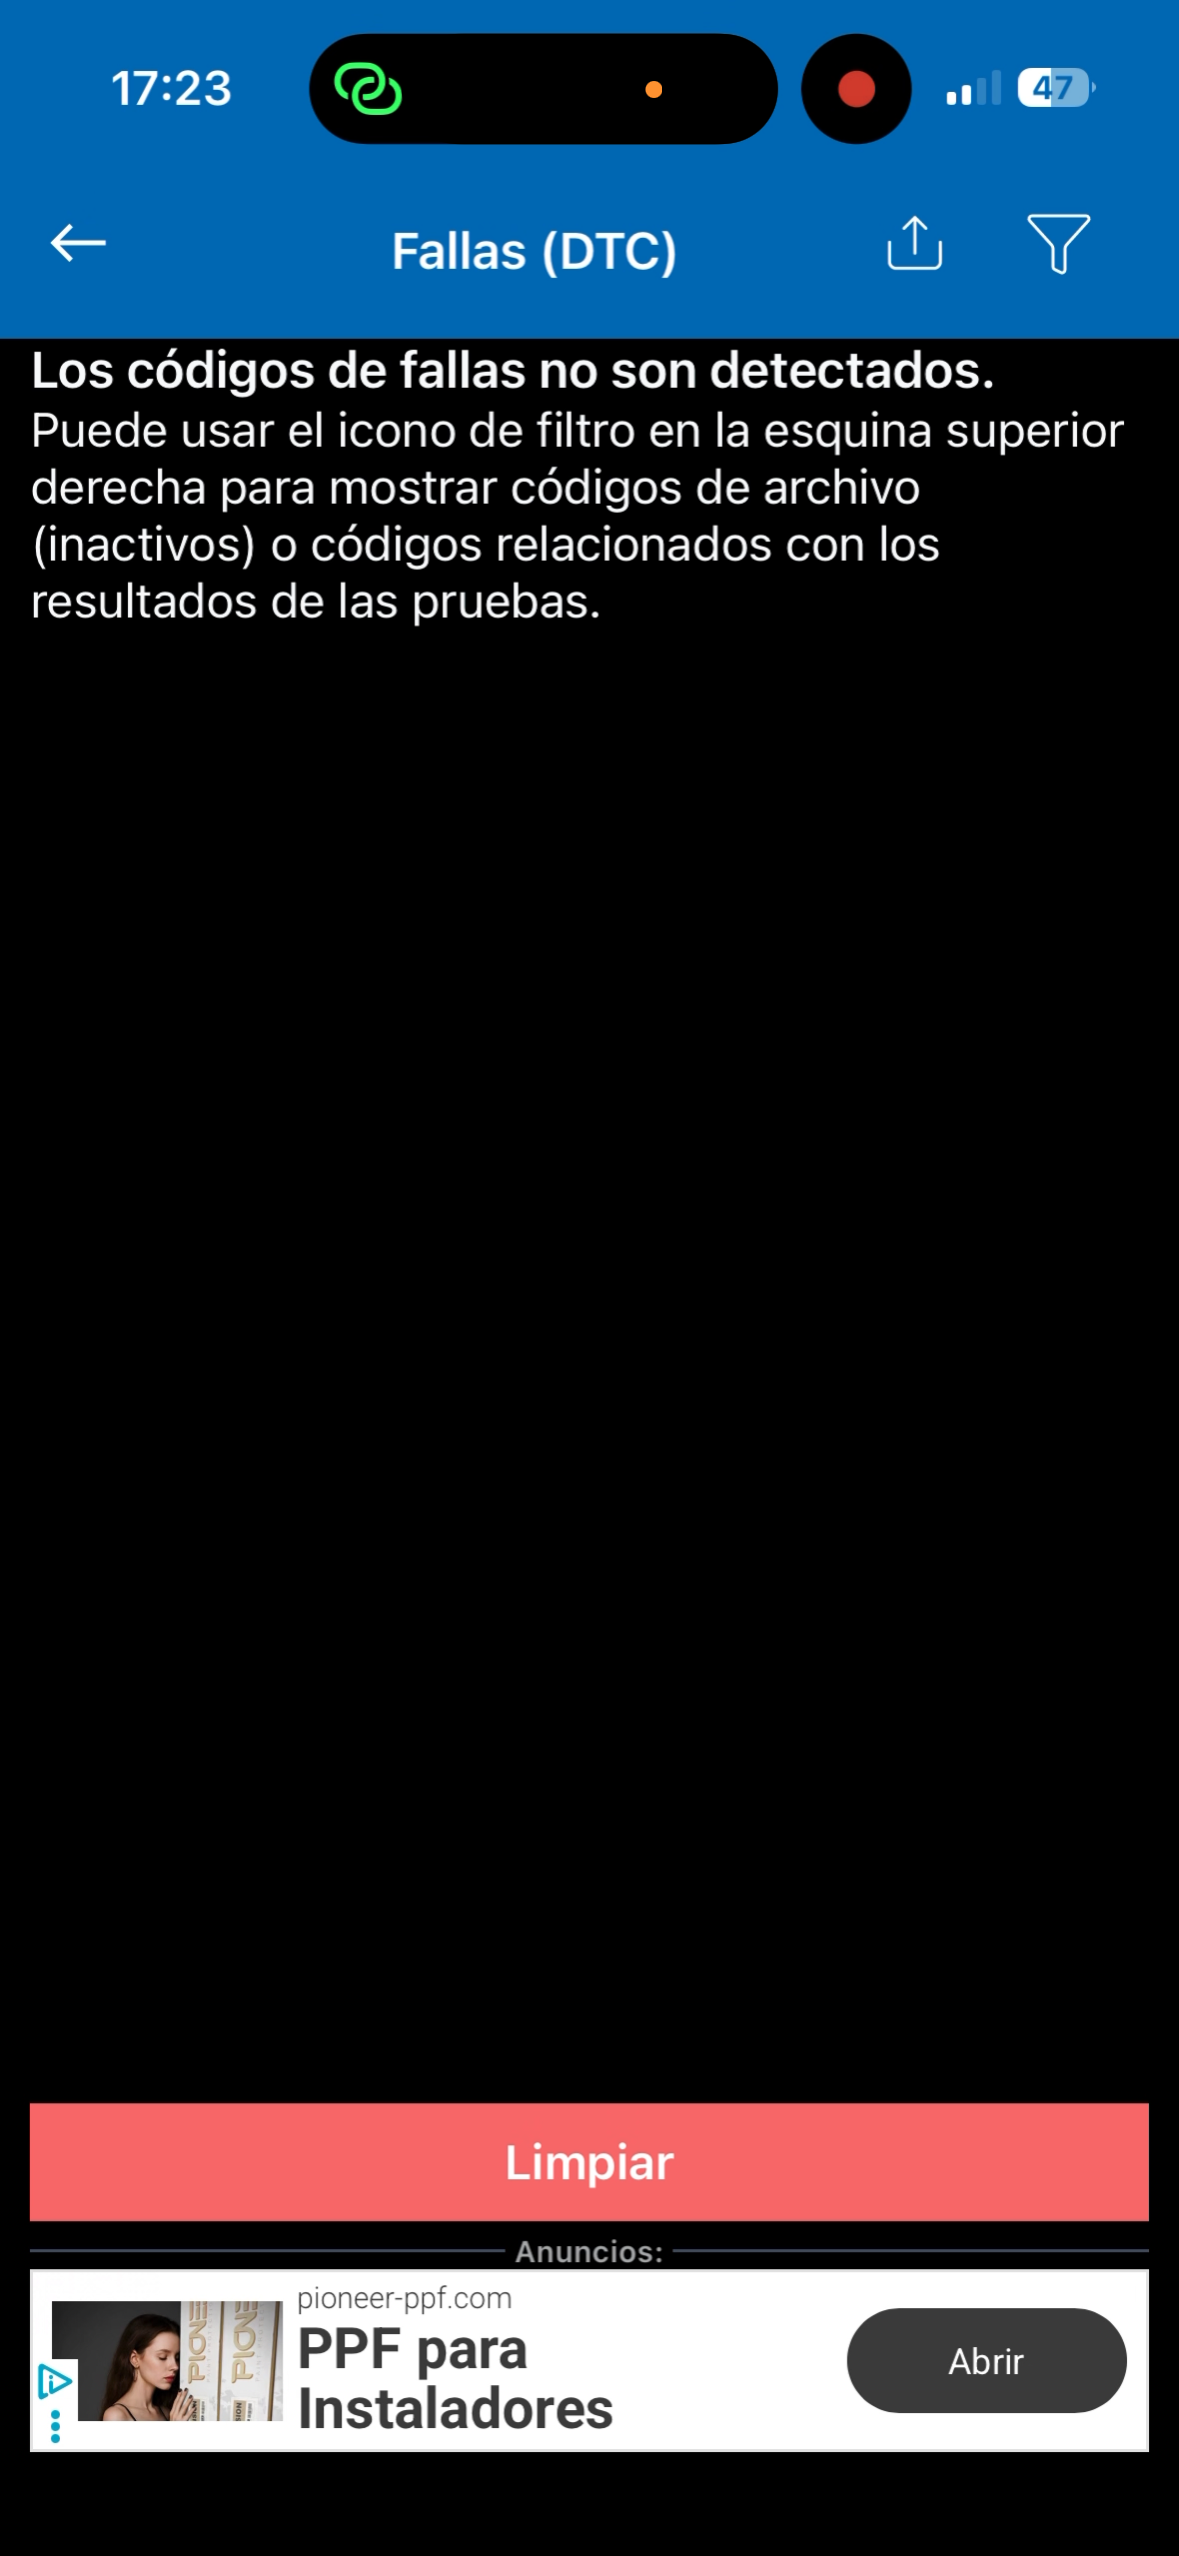
\includegraphics[height=7cm]{Ilustraciones/opel_konwei.PNG}
\subcaption{Esc\'aner comercial de referencia.}
\label{fig:opel_konwei}
\end{minipage}\hfill
\begin{minipage}[t]{0.32\textwidth}
\centering
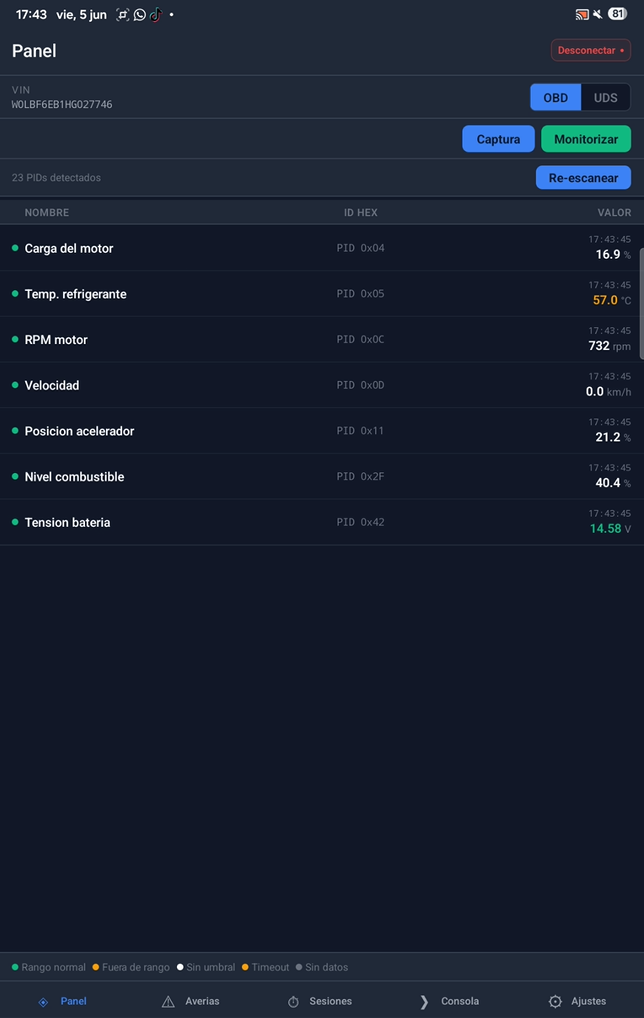
\includegraphics[height=7cm]{Ilustraciones/opel_panel.png}
\subcaption{Panel de telemetr\'ia.}
\label{fig:opel_panel}
\end{minipage}\hfill
\begin{minipage}[t]{0.32\textwidth}
\centering
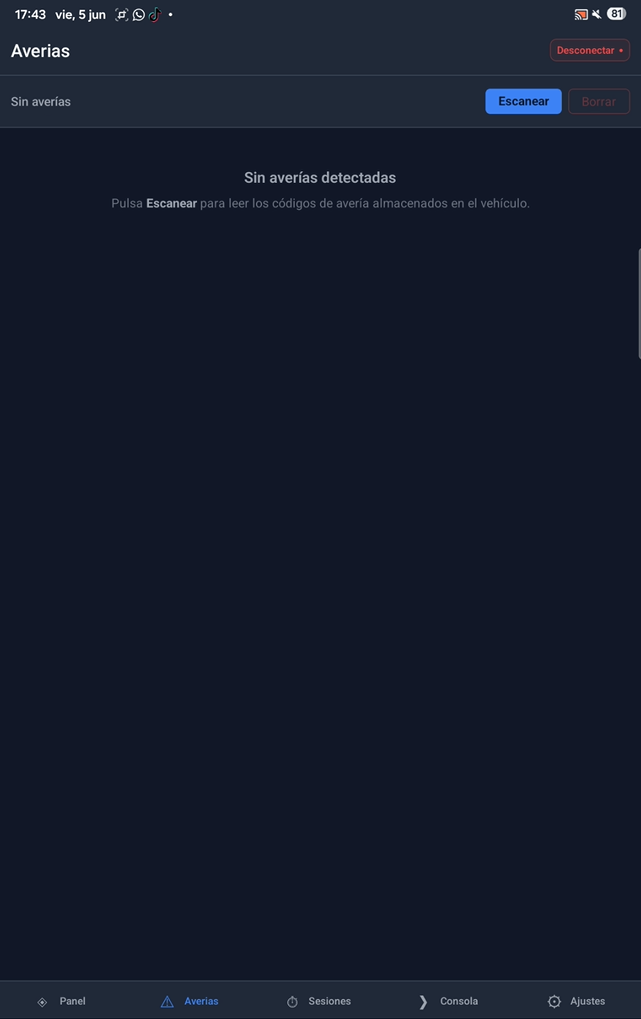
\includegraphics[height=7cm]{Ilustraciones/opel_dtc.png}
\subcaption{Escaneo de DTCs.}
\label{fig:opel_dtc}
\end{minipage}
\caption{Validación sobre el Opel Astra K: lectura de la herramienta comercial de referencia (a) frente al panel de telemetría (b) y el escaneo de DTCs (c) de la herramienta desarrollada.}
\label{fig:opel_astra}
\end{figure}



\section{Validación funcional del protocolo OBD-II}
\label{sec:resultados_protocolo}

La herramienta de diagnóstico fue capaz de completar satisfactoriamente el ciclo completo de consulta para los 25 PIDs implementados en el modo 0x01, la lectura del VIN del modo 0x09 (mediante la secuencia multi-frame), los modos de gestión de DTCs 0x03 y 0x04, y los servicios UDS 0x10 (DiagnosticSessionControl) y 0x22 (ReadDataByIdentifier).

La tabla~\ref{tab:pids_validados} resume los parámetros validados más representativos, indicando el PID, la fórmula de decodificación aplicada y el rango de valores observados durante las sesiones de prueba.

\begin{table}[!htbp]
\caption{PIDs del modo 0x01 validados en el banco de ensayo.}
\label{tab:pids_validados}
\centering
\renewcommand{\arraystretch}{1.2}
\begin{tabular}{|c|l|l|c|}
\hline
\textbf{PID} & \textbf{Parámetro} & \textbf{Fórmula (A, B = bytes de respuesta)} & \textbf{Rango observado} \\
\hline
\texttt{0x0C} & RPM del motor & $((A \times 256) + B) / 4$ & 800 -- 6000\,rpm \\
\texttt{0x0D} & Velocidad & $A$ & 0 -- 255\,km/h \\
\texttt{0x05} & Temp. refrigerante & $A - 40$ & 15 -- 95\,°C \\
\texttt{0x0F} & Temp. aire admisión & $A - 40$ & 15 -- 45\,°C \\
\texttt{0x0A} & Presión combustible & $A \times 3$ & 240 -- 360\,kPa \\
\texttt{0x11} & Posición acelerador & $A \times 100 / 255$ & 0 -- 100\,\% \\
\texttt{0x04} & Carga calculada motor & $A \times 100 / 255$ & 10 -- 85\,\% \\
\texttt{0x5E} & Consumo combustible & $((A \times 256) + B) / 20$ & 0,4 -- 8,5\,L/h \\
\texttt{0x42} & Tensión de batería & $((A \times 256) + B) / 1000$ & 12,4 -- 14,8\,V \\
\hline
\end{tabular}
\end{table}

La respuesta VIN se validó con una cadena de 17 caracteres ASCII, verificando que la secuencia ISO-TP multi-frame (FF + FC + CF $\times$ 2) se completaba correctamente en el 100\% de los intentos realizados con el bus en modo determinista. El VIN reconstruido en la herramienta Python coincidió en todos los casos con la cadena configurada en el simulador Arduino.

El ciclo de gestión de DTCs se validó íntegramente: lectura de lista vacía, inyección de los tres DTCs del conjunto (\texttt{P0300}, \texttt{P0171}, \texttt{P0420}) mediante la interrupción hardware del pin D4, lectura de la lista con los códigos presentes, borrado y confirmación de lista vacía. La codificación J2012 de los DTCs fue correcta en todos los casos.


% TODO - verificar que los números de latencia son reales (medidos), no estimados
\section{Métricas de rendimiento de la comunicación}
\label{sec:resultados_rendimiento}

Se midió la latencia extremo a extremo de una consulta OBD-II completa, desde el envío del comando JSON desde la aplicación móvil hasta la recepción de la respuesta decodificada, en condiciones de bus sin ruido. Las mediciones se realizaron sobre 100 consultas consecutivas del PID \texttt{0x0C} (RPM).

Los resultados obtenidos se resumen en la tabla~\ref{tab:latencias}:

\begin{table}[!htbp]
\caption{Latencia extremo a extremo de una consulta OBD-II (100 muestras, bus en modo determinista).}
\label{tab:latencias}
\centering
\renewcommand{\arraystretch}{1.2}
\begin{tabular}{|l|c|}
\hline
\textbf{Componente} & \textbf{Latencia media (ms)} \\
\hline
BLE Write (app → Raspberry Pi) & 12 -- 25 \\
Procesamiento JSON + construcción trama & $< 1$ \\
Transacción ISO-TP CAN (SF) & 2 -- 8 \\
Decodificación + logging SQLite & 3 -- 7 \\
BLE Notify (Raspberry Pi → app) & 10 -- 20 \\
\hline
\textbf{Total extremo a extremo} & \textbf{28 -- 62} \\
\hline
\end{tabular}
\end{table}

La latencia dominante en el sistema es la introducida por la capa BLE, que suma las contribuciones del Write y la Notify. La latencia CAN+ISO-TP es despreciable frente a la BLE a las velocidades de bus utilizadas.

En el modo de monitorización continua con cinco PIDs a 500\,ms de periodo, el sistema fue capaz de mantener una tasa de actualización estable sin pérdidas de muestras durante sesiones de 10 minutos. El reenvío de las muestras del hilo de monitorización al cliente BLE no presentó pérdidas ni saturación en ninguno de los ensayos.

\section{Comportamiento ante condiciones de bus realistas y errores}
\label{sec:resultados_ruido}

Se evaluó el comportamiento del sistema con los mecanismos opcionales de variabilidad del simulador activos (\texttt{ADD\_NOISE} y \texttt{BROADCAST\_ENABLE}) y ante respuestas negativas (NRC) de la ECU.

Los resultados más relevantes de estas pruebas son:

\begin{itemize}
    \item \textbf{Tramas de difusión}: Con \texttt{BROADCAST\_ENABLE} activo, las tramas no solicitadas (identificadores \texttt{0x280}, \texttt{0x320} y \texttt{0x3D0}) fueron ignoradas por la pila \texttt{can-isotp}, que solo entrega los mensajes dirigidos a la dirección de respuesta de la ECU (\texttt{0x7E8}). En ningún caso una trama de difusión se interpretó como respuesta válida a una petición.

    \item \textbf{Ruido en los sensores}: Con \texttt{ADD\_NOISE} activo, los valores de telemetría presentaron el \textit{jitter} esperado dentro de sus rangos físicos, sin afectar a la correcta decodificación de las respuestas ni a la estabilidad de la monitorización continua.

    \item \textbf{Respuestas negativas UDS}: Las respuestas NRC (por ejemplo, \texttt{0x22} al leer un DID propietario fuera de la sesión extendida) fueron detectadas y registradas correctamente. El hilo de monitorización omite la muestra afectada y prosigue con el siguiente PID del ciclo, sin bloquear la sesión.

    \item \textbf{Robustez del transporte}: El timeout de recepción de 5\,segundos y el reensamblado automático de \texttt{can-isotp} absorbieron la latencia de las transmisiones multi-frame sin generar falsos errores, manteniendo la sesión estable durante toda la prueba.
\end{itemize}

La Figura~\ref{fig:res_consolas} muestra la traza de ejecución durante una de estas pruebas: la consola del simulador Arduino, que emite las tramas de difusión y el ruido inyectado en los sensores, y la consola de la Raspberry Pi, donde la pila \texttt{can-isotp} descarta las tramas ajenas y decodifica únicamente las respuestas dirigidas a la dirección de la ECU.

\begin{figure}[H]
\centering
\begin{minipage}[t]{0.48\textwidth}
\centering
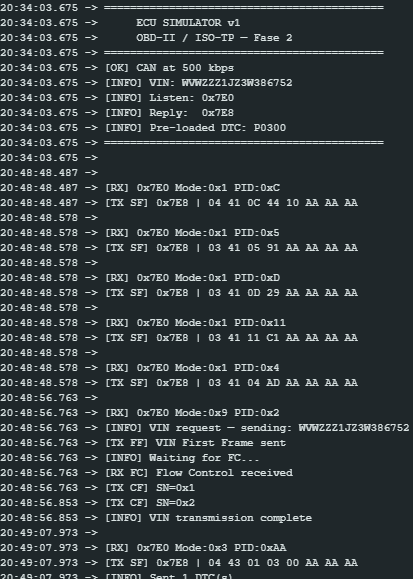
\includegraphics[height=7.5cm]{Ilustraciones/iter_2_ard.png}
\subcaption{Consola del simulador Arduino.}
\label{fig:res_consola_ard}
\end{minipage}\hfill
\begin{minipage}[t]{0.48\textwidth}
\centering
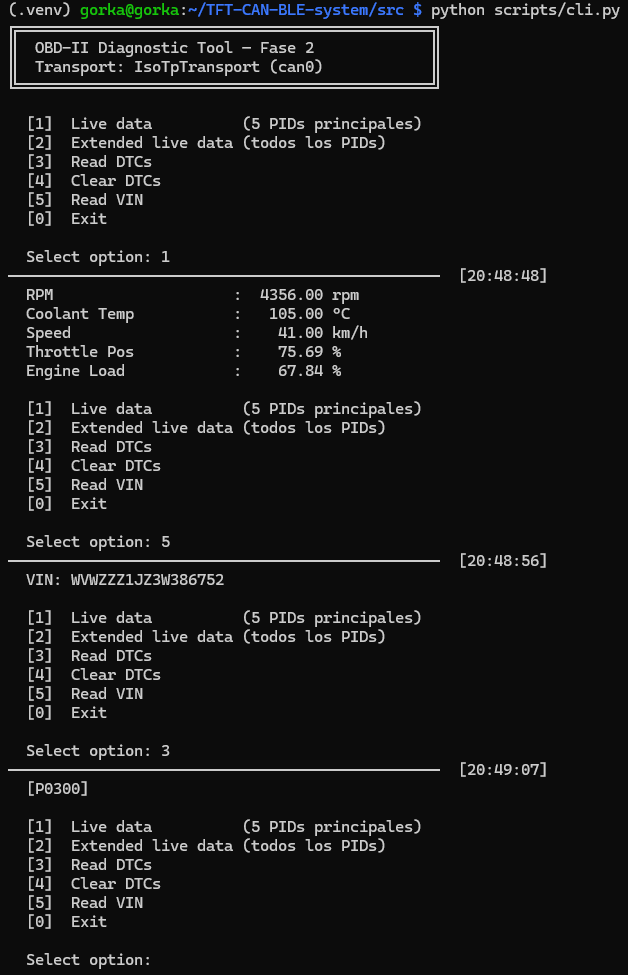
\includegraphics[height=7.5cm]{Ilustraciones/iter_2_pi.png}
\subcaption{Consola de la Raspberry Pi.}
\label{fig:res_consola_pi}
\end{minipage}
\caption{Traza de ejecución bajo condiciones de bus realistas: consola del simulador Arduino emitiendo tramas de difusión y ruido (a) y consola de la Raspberry Pi filtrando y decodificando las respuestas válidas (b).}
\label{fig:res_consolas}
\end{figure}

\section{Interfaz de la aplicación móvil}
\label{sec:resultados_app}

A continuación se recogen las capturas de las distintas pantallas de la aplicación móvil obtenidas durante las pruebas en el vehículo real, que ilustran el resultado final de la interfaz de usuario sobre las cinco pestañas de navegación y el flujo de conexión.

\begin{figure}[H]
\centering
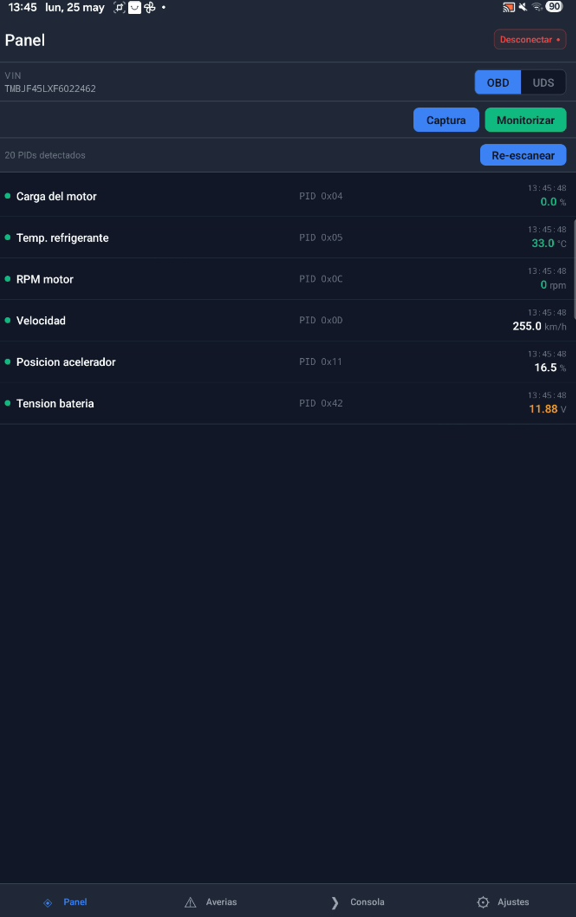
\includegraphics[height=9cm]{Ilustraciones/datos_real.png}%
\hspace{0.04\textwidth}%
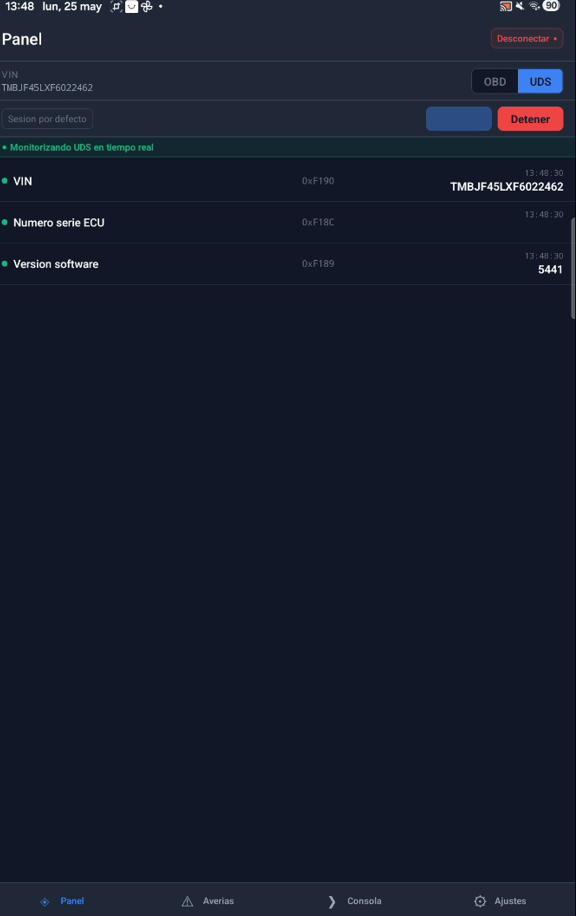
\includegraphics[height=9cm]{Ilustraciones/uds_real.png}
\caption{Pantalla \textit{Panel}: telemetría en tiempo real (izquierda) y pestaña UDS con control de sesión y lectura de DIDs (derecha).}
\label{fig:res_app_panel}
\end{figure}

\begin{figure}[H]
\centering
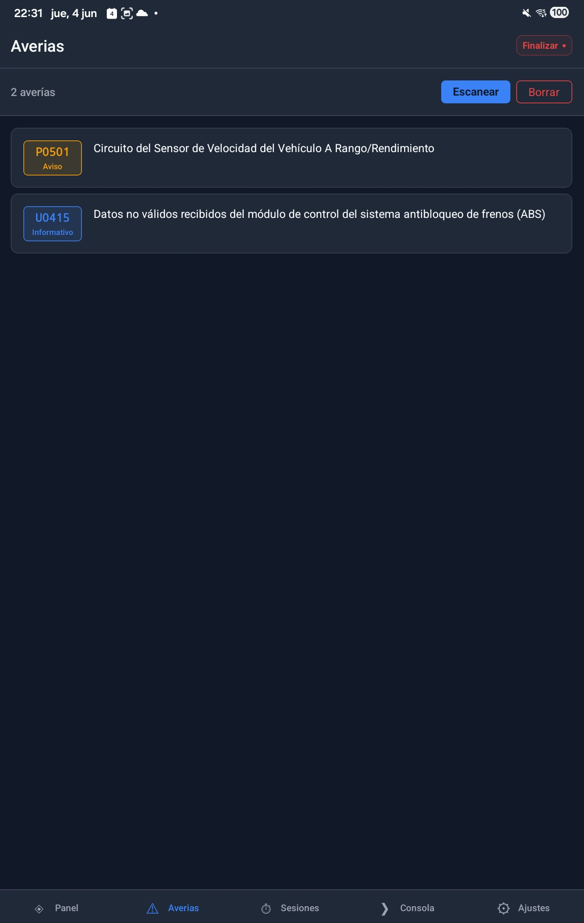
\includegraphics[height=9cm]{Ilustraciones/dtcs_real.png}%
\hspace{0.04\textwidth}%
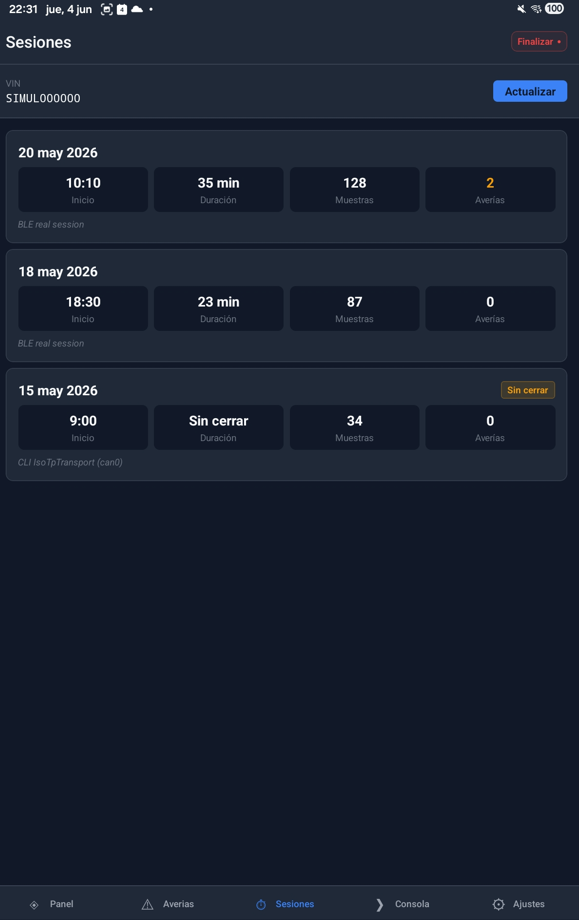
\includegraphics[height=9cm]{Ilustraciones/sesiones_sim.png}
\caption{Pantallas \textit{Averías} (izquierda), con la lista de DTCs leídos de la ECU, y \textit{Sesiones} (derecha), con el historial de sesiones almacenado en SQLite.}
\label{fig:res_app_dtc_sesiones}
\end{figure}

\begin{figure}[H]
\centering
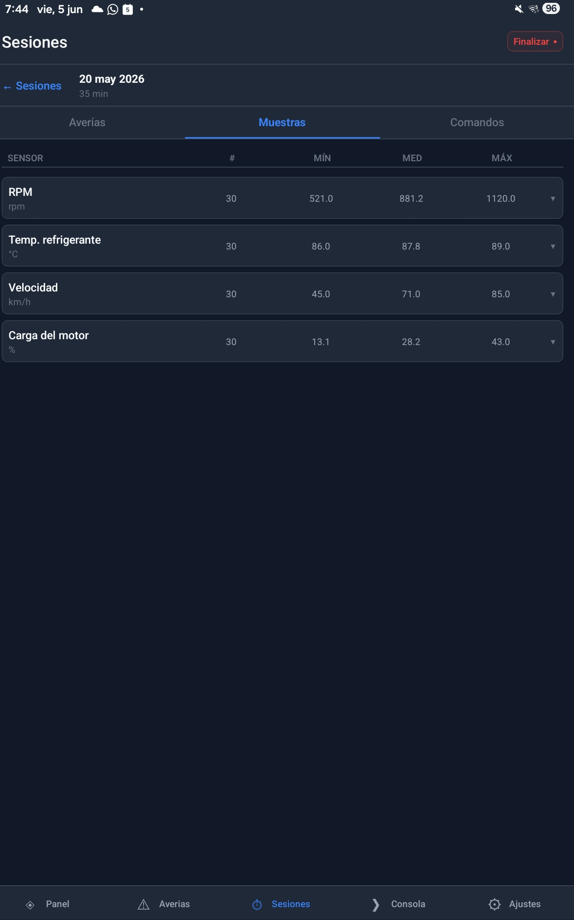
\includegraphics[height=9cm]{Ilustraciones/sesion_detalle.png}%
\hspace{0.04\textwidth}%
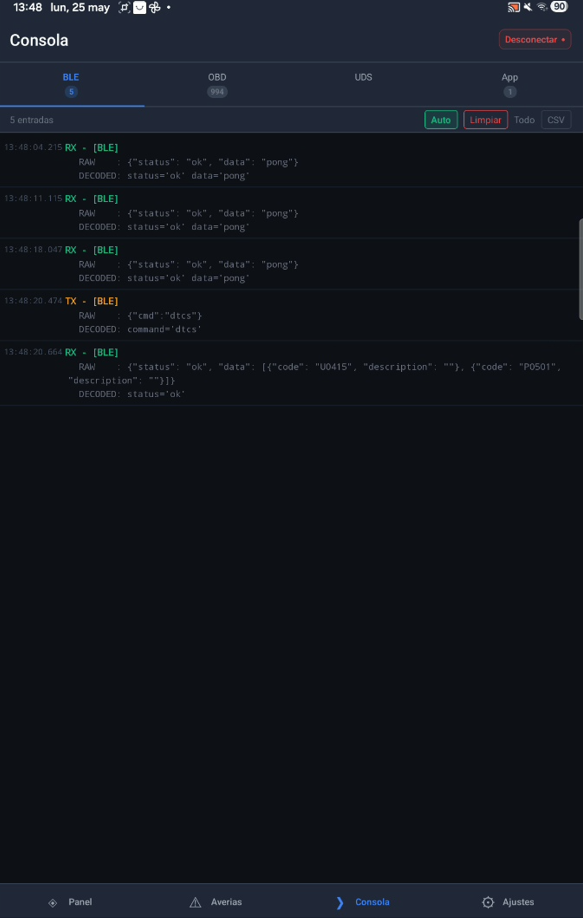
\includegraphics[height=9cm]{Ilustraciones/logs_real.png}
\caption{Detalle de una sesión con las muestras agrupadas por sensor (izquierda) y pantalla \textit{Consola} con el envío de comandos JSON y el registro de comunicación BLE (derecha).}
\label{fig:res_app_detalle_consola}
\end{figure}

\begin{figure}[H]
\centering
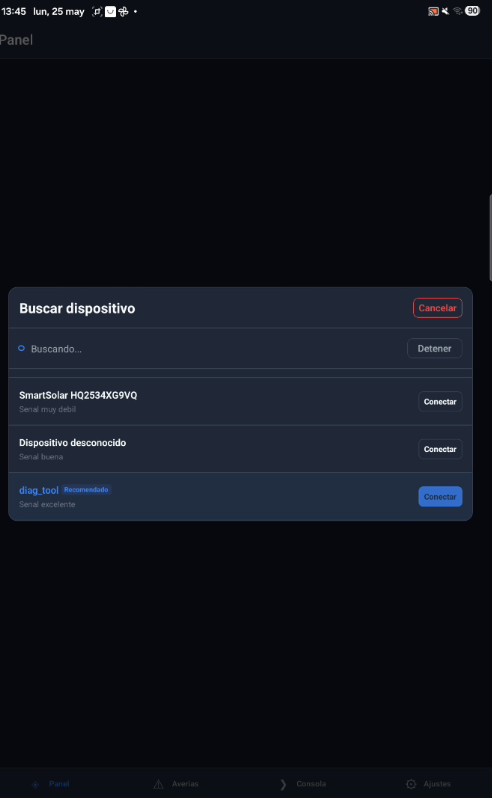
\includegraphics[height=9cm]{Ilustraciones/conexion.png}%
\hspace{0.04\textwidth}%
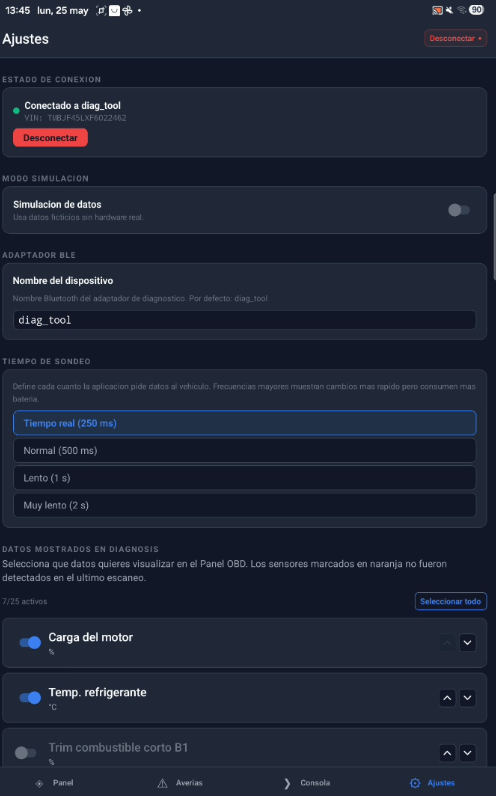
\includegraphics[height=9cm]{Ilustraciones/ajustes.png}
\caption{Pantalla \textit{Ajustes} (izquierda), con la gestión de conexión y el modo de simulación, y la pantalla de ajustes (derecha).}
\label{fig:res_app_ajustes_conexion}
\end{figure}

% TODO - revisar y redactar
\section{Grado de consecución de los objetivos}
\label{sec:resultados_objetivos}

La tabla~\ref{tab:objetivos} recoge el grado de consecución de cada uno de los objetivos específicos definidos en la Sección~\ref{sec:objetivos}, evaluado sobre la base de los resultados de las pruebas de integración.

\begin{table}[H]
\caption{Evaluación del grado de consecución de los objetivos específicos.}
\label{tab:objetivos}
\centering
\renewcommand{\arraystretch}{1.2}
\begin{tabular}{|l|p{7cm}|c|}
\hline
\textbf{Obj.} & \textbf{Indicador de consecución} & \textbf{Resultado} \\
\hline
O1 & Pila ISO-TP + OBD-II modos 0x01/03/04/09 operativa & Completo \\
O2 & Simulador Arduino responde a los 4 modos con datos realistas & Completo \\
O3 & Servicios UDS (0x10/0x22) y mecanismos opcionales de ruido/difusión & Completo \\
O4 & Servidor BLE GATT con NUS operativo en Raspberry Pi & Completo \\
O5 & App React Native Android/iOS con 5 pantallas funcionales & Completo \\
O6 & Logging SQLite con sesiones, muestras y comandos & Completo \\
\hline
\end{tabular}
\end{table}

Los seis objetivos específicos se han alcanzado en su totalidad. La validación sobre vehículo real (Sección~\ref{sec:resultados_vehiculo_real}) confirmó la compatibilidad del sistema con ECUs de producción, completando la cadena de validación desde el banco de ensayo controlado hasta un entorno vehicular real.
